% !TeX spellcheck = ru_RU
% !TEX root = vkr.tex

%\section{Тестирование}
%%Основной трудностью при отладке и тестировании IP-ядра является извлечение данных из ПЛИС в требуемый момент времени. 
%Для проверки корректности работы разработанного IP-ядра Vivado IDE предоставлет набор штатных средств, таких как симуляция и интегрированный логический анализатор (IP-ядро ILA).
%
%\subsection{Симуляция}
%Первым механизмом проверки IP-ядра является симуляция. Vivado IDE позволяет выполнить 5 различных видов симуляций. Отличием симуляций является формат представления тестируемого объекта и совокупность учитываемых задержек распространения сигнала. Главным образом используются следующие два вида симуляций.
%\begin{enumerate}
%    \item behaveariol simulation -- объект представлен в виде HDL-кода, задержки не учитываются.
%    \item post-implementation timimng simulation -- объект представлен в виде размещенного набора синтезированных примитивов, учитываются задержки распространения сигнала в соединениях, а также задержки самих примитивов.
%\end{enumerate}
%Первая симуляция является наиболее простой, а последнея -- наиболее строгой. Симуляции наиболее активно используются при разработке IP-ядра и его промежуточной отладке.
%
%\subsection{ILA}
%Для проверки работоспособности обнаружителя размещенного в ПЛИС, следует использовать готовое IP-ядро под названием Integrated Logic Analyzer (ILA)\cite{ila}. Данный блок можно воспринимать как программный осциллограф, который при срабатывании триггера выполняет отписывание набора сигналов и передачу собранных данных на ПК. Для использования этого IP-ядра, его необходимо добавить в VHDL-код отлаживаемой системы и подключить к его входам интересующие линии данных. Полученную схему необходимо повторно синтезировать и разместить на ПЛИС, поэтому перед использованием ILA рекомендуется прописать ограничения на размещение синтезированных примитивов (placement constraints). В противном случае добавление ILA может повлиять на расположение прочих синтезированных примитивов и нарушить спроектированный до этого VHDL-дизайн.




\section{Тестирование}

Проверка корректности функционирования ПЛИС-обнаружителя выполнялась в среде 
Vivado
с использованием режима behavioral simulation. Данный режим моделирования позволяет проверить логическую корректность реализации на уровне RTL-описания без учёта временных задержек, вносимых после этапов синтеза и трассировки.

\subsection{Параметры тестовой симуляции}

Для проведения моделирования был сформирован тестовый комплексный сигнал с частотой дискретизации
\[
f_s = 100\ \text{кГц},
\]
соответствующей режиму работы системы после децимации. Сигнал моделировал поток отсчётов АЦП и содержал три копии эталонной преамбулы, распределённые во времени.

В сигнал была внесена искусственная частотная ошибка
\[
f_{\text{err}} = -2800\ \text{Гц}.
\]

Размер БПФ, используемый в архитектуре обнаружителя,
\[
N_{\text{FFT}} = 2048,
\]
что определяет частотное разрешение
\[
\Delta f = \frac{f_s}{N_{\text{FFT}}} \approx 48.828125\ \text{Гц}.
\]

Частотные гипотезы формировались на основе циклического сдвига спектра преамбулы.  
Первый частотный сдвиг выбирался как ближайший к истинной частотной ошибке.  
Три последующих сдвига выбирались последовательно дальше от истинного значения ошибки с целью наблюдения деградации корреляционного пика при увеличении остаточной частотной рассинхронизации.

Таким образом обеспечивалась возможность экспериментально продемонстрировать:
\begin{itemize}
\item уменьшение амплитуды корреляционного пика при росте остаточной частотной ошибки;
\item исчезновение отчётливо выраженного максимума при превышении допустимого уровня рассогласования.
\end{itemize}

Значения использованных частотных сдвигов составили:

\[
[-2783.203125,\ -2734.375,\ -2685.546875,\ -2636.71875]\ \text{Гц}.
\]

Основные параметры тестовой симуляции приведены в таблице~\ref{tab:simulation_params}.

\begin{table}[h]
\centering

\begin{tabular}{|l|c|}
	\hline
	\rowcolor{green!25}
	Параметр & Значение \\
	\hline
	Частота дискретизации $f_s$ & 100 кГц \\
	Размер БПФ $N_{\text{FFT}}$ & 2048 \\
	Частотное разрешение $\Delta f$ & 48.828125 Гц \\
	Внесённая частотная ошибка $f_{\text{err}}$ & -2800 Гц \\
	Количество преамбул в тестовом сигнале & 3 \\
	Количество частотных гипотез & 4 \\
	Значения частотных сдвигов & 
	\begin{tabular}{c}
		-2783.203125 Гц \\
		-2734.375 Гц \\
		-2685.546875 Гц \\
		-2636.71875 Гц
	\end{tabular} \\
	\hline
\end{tabular}
\caption{Параметры тестовой RTL-симуляции}
\label{tab:simulation_params}
\end{table}

\subsection{Организация моделирования}

Спектр эталонной преамбулы был предварительно вычислен в среде Python. На его основе были сформированы файлы инициализации памяти формата \texttt{.coe}, использованные для загрузки данных в BRAM модуля \texttt{reference\_reader}.  

Аналогичным образом входной тестовый сигнал, имитирующий поток отсчётов АЦП, был подключён к входу обнаружителя в составе тестового окружения.

В ходе behavioral simulation:
\begin{itemize}
\item выполнялось формирование перекрывающихся блоков длиной 2048 отсчётов;
\item осуществлялось прямое БПФ, спектральное умножение и обратное БПФ;
\item результаты расчёта взаимнокорреляционной функции сохранялись во внешний файл.
\end{itemize}

Сохранённые данные обрабатывались Python-скриптом, который выполнял визуализацию корреляционных функций для всех частотных гипотез и сравнение с результатами, полученными полностью в программной модели.

\subsection{Результаты}

Для первой частотной гипотезы, выбранной как ближайшая к истинной частотной ошибке, наблюдались три отчётливых корреляционных пика, соответствующих числу преамбул, встроенных в тестовый сигнал.  

Для второй гипотезы, характеризующейся несколько большей остаточной частотной ошибкой, также сохранялись три различимых корреляционных пика, однако их амплитуда была заметно ниже по сравнению с первой гипотезой. Это отражает частичную потерю когерентности при увеличении частотного рассогласования.

Для третьей и четвёртой частотных гипотез выраженные корреляционные максимумы уже не наблюдались. Выходной сигнал имел шумоподобный характер без отчётливо выделяющихся пиков, что свидетельствует о превышении допустимого уровня остаточной частотной ошибки, при котором энергия корреляционного отклика рассеивается и не формирует локального максимума.

\begin{figure}[h]
\centering
 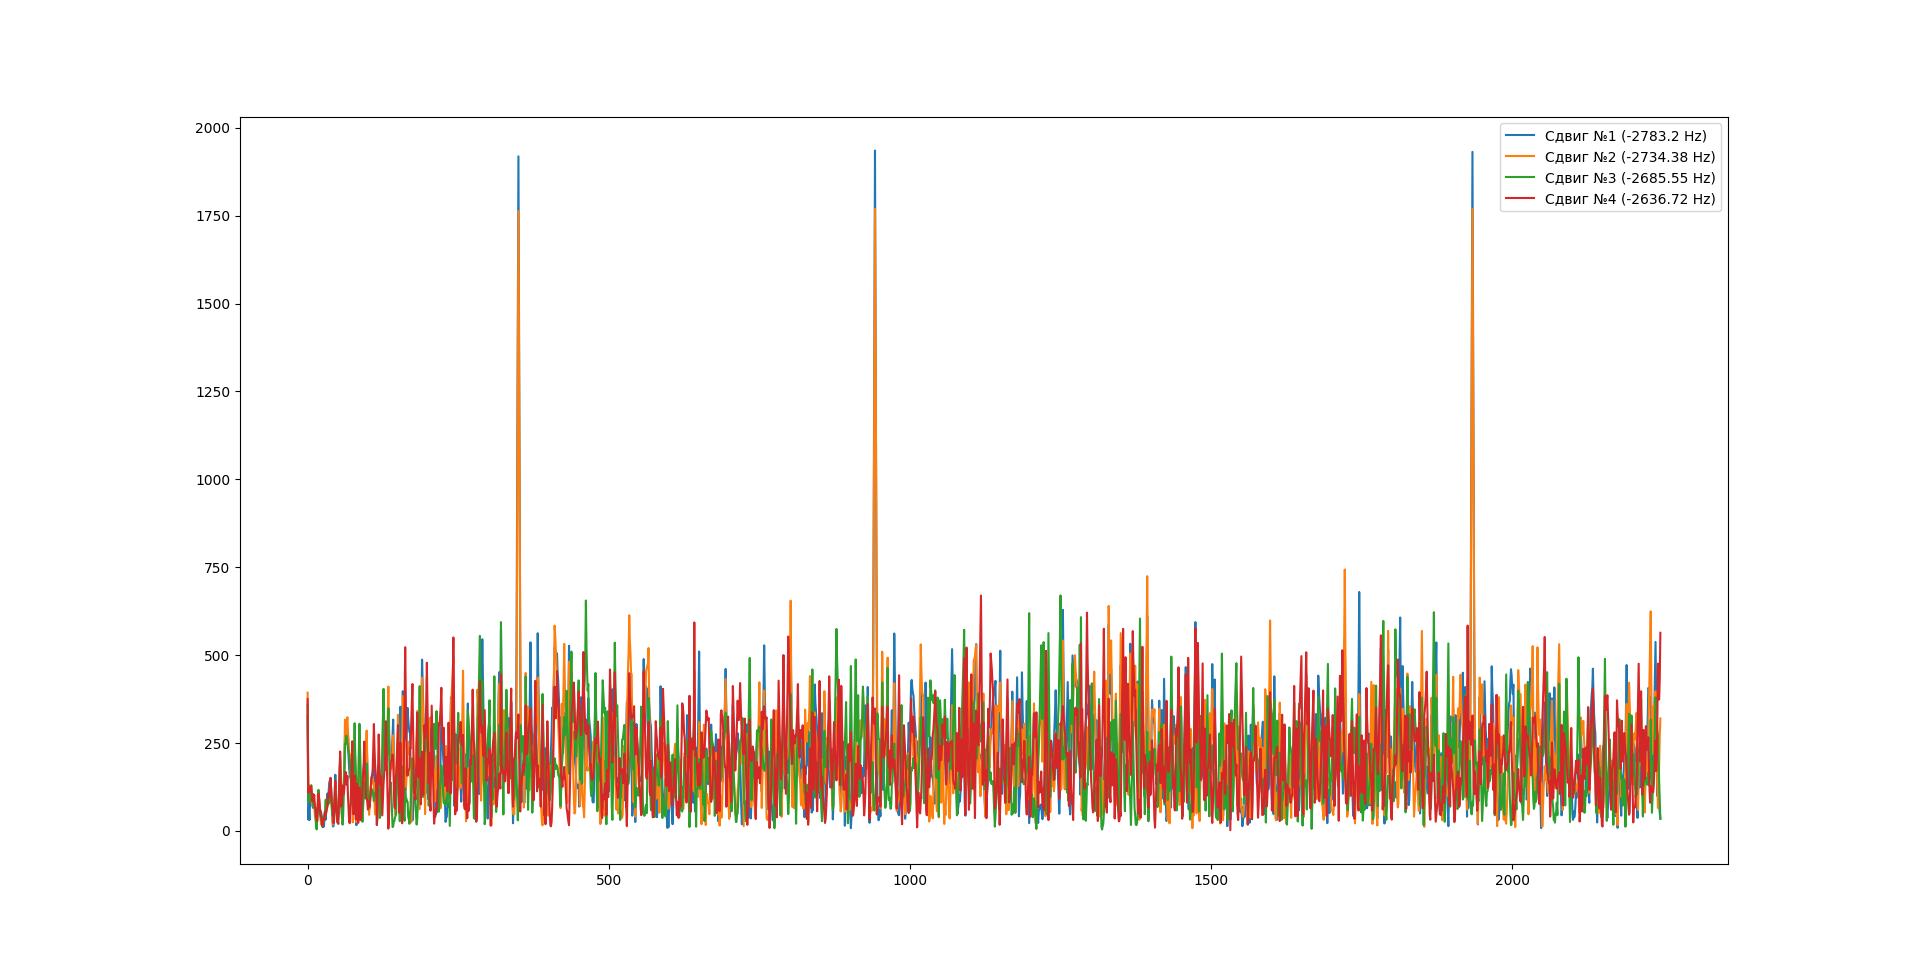
\includegraphics[
 	width=\textwidth,
 	trim=4.5cm 2cm 4cm 2.5cm,
 	clip
 ]{pics/vivado_corr.png}
\caption{Корреляционные функции для четырёх частотных гипотез}
\label{fig:correlation_all}
\end{figure}

%\begin{figure}[h]
%\centering
%% \includegraphics[width=\textwidth]{correlation_degradation.png}
%\caption{Деградация корреляционного пика при увеличении остаточной частотной ошибки}
%\label{fig:correlation_degradation}
%\end{figure}

Полученные результаты полностью совпали с расчётами, выполненными в программной модели, что подтверждает функциональную корректность реализации алгоритма корреляции и механизма обработки частотных гипотез на уровне RTL-описания.





%\section{Тестирование}
%
%Проверка корректности функционирования ПЛИС-обнаружителя выполнялась средствами RTL-моделирования в среде Vivado. В рамках работы использовалась исключительно \textit{behavioral simulation}, позволяющая проверить логическую корректность реализации без учёта временных задержек, вносимых после синтеза и трассировки.
%
%\subsection{Подготовка тестовых данных}
%
%Для проведения симуляции был заранее сформирован набор комплексных отсчётов сигнала с частотой дискретизации
%\[
%f_s = 100\ \text{кГц},
%\]
%что соответствует режиму работы системы после децимации.
%
%Тестовый сигнал моделировал работу АЦП приемника и содержал несколько копий эталонной преамбулы, распределённых во времени. Всего в сигнал было встроено три преамбулы.  
%
%В сигнал дополнительно была внесена фиксированная частотная ошибка:
%\[
%f_{\text{err}} = -2800\ \text{Гц}.
%\]
%
%Размер БПФ, используемый в архитектуре обнаружителя, равен
%\[
%N_{\text{FFT}} = 2048.
%\]
%
%Частотное разрешение одного спектрального отсчёта определяется выражением:
%\[
%\Delta f = \frac{f_s}{N_{\text{FFT}}} = \frac{100000}{2048} \approx 48.828125\ \text{Гц}.
%\]
%
%\subsection{Формирование частотных гипотез}
%
%Спектр эталонной преамбулы был вычислен заранее в среде Python. Для реализации поиска с компенсацией частотной ошибки использовался метод циклического сдвига спектра.
%
%На основе частотного разрешения $\Delta f$ были выбраны четыре частотных сдвига, ближайшие к внесённой частотной ошибке. Их значения составили:
%
%\[
%[-2783.203125,\ -2734.375,\ -2685.546875,\ -2636.71875]\ \text{Гц}.
%\]
%
%Указанные значения соответствуют дискретным спектральным сдвигам, кратным $\Delta f$.  
%
%Таким образом, среди выбранных гипотез две являются наиболее близкими к реальной частотной ошибке $f_{\text{err}} = -2800$ Гц, а две остальные имеют большее рассогласование.
%
%На основе рассчитанных спектров были сформированы файлы инициализации памяти формата \texttt{.coe}, используемые в Vivado для загрузки данных в блочную память (BRAM). Спектры преамбул были загружены в модуль \texttt{reference\_reader}.  
%
%Аналогичным образом входной тестовый сигнал, имитирующий поток отсчётов АЦП, был подготовлен и подключён к входу проектируемого обнаружителя в составе тестового окружения.
%
%\subsection{Проведение RTL-симуляции}
%
%После подготовки входных данных и инициализации BRAM была выполнена behavioral simulation проекта.  
%
%В процессе моделирования:
%\begin{itemize}
%	\item входной поток комплексных отсчётов подавался на тракт корреляционной обработки;
%	\item выполнялось формирование перекрывающихся блоков длиной 2048 отсчётов;
%	\item осуществлялось прямое БПФ, спектральное умножение и обратное БПФ;
%	\item результаты взаимнокорреляционной функции сохранялись во внешний файл.
%\end{itemize}
%
%Сохранённые данные затем обрабатывались Python-скриптом, который:
%\begin{itemize}
%	\item считывал результаты моделирования;
%	\item визуализировал корреляционные функции для всех частотных гипотез;
%	\item выполнял сравнение с эталонными расчётами, выполненными полностью в программной модели.
%\end{itemize}
%
%\subsection{Результаты моделирования}
%
%В результате анализа было установлено, что:
%
%\begin{itemize}
%	\item для двух частотных сдвигов, наиболее близких к реальной частотной ошибке $-2800$ Гц, наблюдаются три отчётливых корреляционных пика;
%	\item число пиков соответствует количеству преамбул, встроенных в тестовый сигнал;
%	\item для двух остальных частотных гипотез выходной сигнал имеет шумовой характер без выраженных максимумов.
%\end{itemize}
%
%Такое поведение полностью соответствует ожидаемому: при существенном частотном рассогласовании энергия корреляционного отклика распределяется и не формирует выраженного максимума.
%
%Результаты RTL-моделирования совпали с результатами расчётов, выполненных в Python, как по положению пиков во времени, так и по их относительной амплитуде.
%
%\begin{figure}[h]
%	\centering
%	% \includegraphics[width=\textwidth]{correlation_all_shifts.png}
%	\caption{Результаты расчёта взаимнокорреляционной функции для четырёх частотных гипотез}
%	\label{fig:correlation_all}
%\end{figure}
%
%\begin{figure}[h]
%	\centering
%	% \includegraphics[width=\textwidth]{correlation_best_shift.png}
%	\caption{Фрагмент корреляционной функции для частотной гипотезы, ближайшей к реальной ошибке}
%	\label{fig:correlation_best}
%\end{figure}
%
%\subsection{Выводы по результатам RTL-симуляции}
%
%Behavioral simulation подтвердила корректность:
%\begin{itemize}
%	\item реализации алгоритма корреляции через БПФ;
%	\item схемы перекрытия блоков (overlap-save);
%	\item механизма обработки нескольких частотных гипотез;
%	\item организации потоков данных внутри архитектуры.
%\end{itemize}
%
%Совпадение результатов аппаратной модели и программного расчёта свидетельствует о функциональной корректности разработанного ПЛИС-обнаружителя на уровне RTL-описания.

%\subsection{Тестовое окружение}
%Разработанный обнаружитель должен удовлетворять предъявляемым к нему требованиям надежности, что означает наличие пропусков сигнала или ложных обнаружений сигнала с частотами не превышающими заданные. Выполнение таких проверок осуществляется на временных интервалах продолжительностью до нескольких дней. Выполнение столь длительных проверок на одной лишь ПЛИС затруднительно. Однако PLutoSDR+ помимо ПЛИС имеет еще и процессор ARM, поэтому для тестирования разработанного обнаружителя будет разумно дополнительно задействовать процессор. PS будет формировать массивы данных и отправлять их в PL на обработку, результаты работы обнаружителя будут возвращены в PS и проанализированы, а ошибки, в случае их наличия, будут зафиксированы.

%\subsubsection{Обмен данными между PS и PL}
%Для реализации рассмотренного сценария требуется механизм обмена данными между PS и PL. Такой механизм может быть реализован на основе DMA или AXI memory-mapped портов. 
%
%Первым вариантом реализации такого механизма, подходящим для потоковой передачи данных, является использование готового IP-ядра AXI DMA\cite{dma}. Данное IP-ядро позволяет как читать данные из PL в PS, так и записывать данные из PS в PL, для чего используются отдельные каналы на чтение и на запись. За счет AXI-портов регистры этого IP-ядра отображаются в адресном пространстве процессора. Для инициирования DMA операций пользователю необходимо выполнить определенную последовательность записей в регистры AXI DMA. На основе информации о регистровой модели[ug на AXI DMA] данного IP-ядра автором был реализован драйвер на языке C, позволяющий выполнять обмен числовыми массивами между PS и PL.
%
%% ВОЗМОЖНО ТУТ ПРИМЕР КОДА ДЛЯ ИНИЦИРОВАНИЯ DMA-ЧТЕНИЯ
%
%Вторым вариантом реализации механизма обмена данных между PS и PL является использование AXI memory-mapped портов. Данный подход используется при создании регистровых моделей и позволяет реализовать собственные протоколы управления для разработанных IP-ядер.

%\subsubsection{Обмен данными между SDR и инструментальной системой}
%При отладке обнаружителя может возникнуть необходимость в построении графиков корреляции и спектра сигнала. Подобные задачи легко решить на Python с использованием numpy и matplotlib\footnote{В репозиториях организации имеется большое количество готового python-кода, предназначенного для отладки алгоритмов ЦОС. В тоже время запуск python-кода на SDR хоть и возможен (проект PYNQ), однако затруднителен и неэффективен т.к. вычислительные мощности инструментальной системы много больше. Поэтому кажется привлекательным отправить данные из SDR на компьтер и проводить отладку там.}. Однако сделать то же самое, написав код на C++ под процессор ARM, крайне затруднительно. Для решения данной задачи был разработан механизм передачи данных между PlutoSDR+ и инструментальной системой. Pluto оснащена USB-C разъемами, которые используются для её подключения к ПК и через которые PLuto может передавать данные по протоколу UART. Таким образом, Pluto может отправлять из PS данные по UART на последовательный порт. В это же время Python-программа, работающая на инструментальной системе, может вычитывать данные из этого же порта. Принятые данные можно обрабатывать и визуализировать требуемым образом. К недостаткам данного подхода можно отнести низкую скорость UART, которая составляет 115200 бод. Однако данной скорости достаточно для передачи численных массивов длиной до нескольких тысяч элементов. При необходимости достижения больших скоростей может быть рассмотрен переход с UART на Ethernet.

% Как мы проверяем, что  всё удачно получилось.  К Новому году для промежуточного отчета желательно хотя бы описать как он будет прово\-диться и на чем.

% Для проверки корректности измерений, выполняемых разработанной системой, был проведен ряд испытаний в рамках которых ПО осуществляло управление стендом, собранного на базе имеющегося парка измерительной аппаратуры и радиотехнического устройства с известными характеристиками. В ходе испытания ПО осуществило измерение параметров целевого устройства. Далее специалистами в области измерений было проверено, соответствуют ли собранные измерения реальным характеристикам радиотехнического устройства.

% \subsection{Описание тестового стенда}
% При разработке системы активно использовался стенд, предназначенный для измерения частотной характеристики фильтра нижних частот. Стенд состоял из генератора ВЧ сигналов, фильтра и анализатора спектра. Полученная частотная характеристика сравнивалась с характеристикой, заявленной производителем данного фильтра. Данный стенд позволял эффективно тестировать и отлаживать систему по следующим причинам.
% \begin{itemize}
%     \item Стенд демонстрирует реальный сценарий использования системы сотрудником для решения задач радиотехнических измерений. Это позволяло получить от коллег, активно работающих с измерительной аппаратурой, обратную связь об удобстве использования данной системы для решения рабочих задач.
%     \item Стенд задействовал два наиболее активно используемых прибора, что позволяло протестировать механизм автоматизированного управления данной аппаратурой.
%     \item Модель такого стенда могла включать в себя программные модули, выполняющие построение графиков и протоколирование результатов. За счет этого можно было отладить работу данных модулей.
% \end{itemize}

% Апробация системы производилась на стенде, предназначенном для производства. Стенд состоял из радиостанции, анализатора спектра и модуля расчета коэффициентов усилителя. Данный стенд выполнял калибровку передатчика радиостанции, производимой организацией. В рамках процедуры калибровки станция настраивается таким образом, чтобы передавать сигнал с мощностью, указанной в спецификации. Станция не подвергнутая калибровке может передавать сигнал с мощностью, значительно отличающейся от заявленной. 

% Радиостанция имеет усилитель, который определяет мощность передаваемого сигнала. Программно записывая в станцию определенные числовые параметры, можно воздействовать на управляющие напряжения, которые контролируют работу усилителя. Однако заранее неизвестно какие значения параметров обеспечат требуемый уровень мощности. Поэтому среди всех возможных значений параметров требовалось найти те, что обеспечивали минимальное отклонение по мощности. 

% \subsection{Результаты}
% В ходе тестирования с использованием первого стенда были учтены замечания коллег и был исправлен ряд ошибок в работе системы. После завершения отладочных мероприятий система успешно выполняла измерения частотной характеристики фильтров нижних частот с разными параметрами.

% В ходе апробации система выполнила процедуру калибровки передатчика для группы радиостанций. Специалистами организации было дано заключение о корректности проведенной калибровки.




% \subsection{Условия эксперимента}
% Железо (если актуально);  версии ОС, компиляторов и параметры командной строки; почему мы выбрали именно эти тесты; входные дан\-ные, на которых проверяем наш подход, и почему мы выбрали именно их.

% \subsection{Исследовательские вопросы }
% По-английски называется \emph{research questions}, в тексте можно ссылаться на них как RQ1, RQ2, и т.~д.
% Необходимо сформулировать, чего мы хотели бы добиться работой (2 пункта будет хорошо):

% \begin{itemize}
% \item Хотим алгоритм, который лучше вот таких-то остальных.
% \item Если в подходе можно включать/выключать составляющие, то насколько существенно каждая составляющая влияет на улучшения.
% \item Если у нас строится приближение каких-то штук, то на сколько точными будут эти приближения.
% \item и т.п.
% \end{itemize}

% Иногда в работах это называют гипотезами, которые потом проверяют. Далее в тексте можно ссылаться на research questions как \textsc{RQ}, это обще\-при\-нятое сокращение.

% \subsection{Метрики}

% Как мы сравниваем, что результаты двух подходов лучше или хуже:
% \begin{itemize}
% \item Производительность.
% \item Строчки кода.
% \item Как часто алгоритм \enquote{угадывает} правильную классификацию входа.
% \end{itemize}

% \noindent Иногда метрики вырожденные (да/нет), это не очень хорошо, но если в области исследований так принято, то ладно.

% \subsection{Результаты}
% Результаты понятно что такое. Тут всякие таблицы и графики, как в таблице \ref{time_cmp_obj_func}. Обратите внимание, как цифры выровнены по правому краю, названия по центру, а разделители $\times$ и $\pm$ друг под другом.

% Скорее всего Ваши измерения будут удовлетворять нормальному распределению, в идеале это надо проверять с помощью критерия Кол\-могорова и т.п.
% Если критерий этого не подтверждает, то у Вас что-то сильно не так с измерениями, надо проверять кэши процессора, отключать Интернет во время измерений, подкручивать среду исполне\-ния (англ. runtime), что\-бы сборка мусора не вмешивалась и т.п.
% Если критерий удовлетворён, то необходимо либо указать мат. ожидание и доверительный/предсказы\-вающий интервал, либо написать, что все измерения проводились с погрешностью, например, в 5\%.
% Замечание: если у вас получится улуч\-шение производительности в пределах погреш\-ности, то это обязательно вызовет вопросы.

% В этом разделе надо также коснуться Research Questions.

% \subsubsection{RQ1} Пояснения
% \subsubsection{RQ2} Пояснения

% \begin{table}
% \def\arraystretch{1.1}  % Растяжение строк в таблицах
% \setlength\tabcolsep{0.2em}
% \centering
% % \resizebox{\linewidth}{!}{%
%     \caption{Производительность какого-то алгоритма при различных разрешениях картинок  (меньше~--- лучше), в мс.,  CI=0.95. За пример таблички кидаем чепчики в честь Я.~Кириленко}
%     \begin{tabular}[C]{
%     S[table-format=4.4,output-decimal-marker=\times]
%     *4{S
%           [table-figures-uncertainty=2, separate-uncertainty=true, table-align-uncertainty=true,
%           table-figures-integer=3, table-figures-decimal=2, round-precision=2,
%           table-number-alignment=center]
%           }
%     }
%     \toprule
%         \multicolumn{1}{r}{Resolution} & \multicolumn{1}{r}{\textsc{TENG}} & \multicolumn{1}{r}{\textsc{LAPM}} &
%         \multicolumn{1}{r}{\textsc{VOLL4}} \\ \midrule
%         1920.1080 & 406.23 \pm 0.94 & 134.06 \pm 0.35 & 207.45 \pm 0.42  \\ \midrule
%         1024.768  & 145.0 \pm 0.47  & 39.68 \pm 0.1   &  52.79  \pm 0.1 \\ \midrule
%         464.848   & 70.57 \pm 0.2   & 19.86 \pm 0.01     & 32.75  \pm 0.04 \\ \midrule
%         640.480   & 51.10 \pm 0.2   & 14.70 \pm 0.1 & 24  \pm 0.04 \\ \midrule
%         160.120   & 2.4 \pm 0.02    & 0.67 \pm 0.01      & 0.92  \pm 0.01 \\
%         \bottomrule
%     \end{tabular}%
% %}
%     \label{time_cmp_obj_func}
% \end{table}

% \clearpage
% \input{bigtable}

% \subsection{Обсуждение результатов}

% Чуть более неформальное обсуждение, то, что сделано. Например, почему метод работает лучше остальных? Или, что делать со случаями, когда метод классифицирует вход некорректно.
